\documentclass[tikz,dvipsnames]{standalone}
\usepackage[utf8]{inputenc}
\usepackage[]{xcolor}
\PassOptionsToPackage{dvipsnames}{xcolor}
\usepackage{amsmath}
\usepackage{amssymb}

\usetikzlibrary{arrows,positioning,shapes}
\usetikzlibrary{decorations.pathreplacing,decorations.markings}
\usetikzlibrary{calc}
% https://tex.stackexchange.com/questions/3161/tikz-how-to-draw-an-arrow-in-the-middle-of-the-line
\tikzset{
  % style to apply some styles to each segment of a path
  on each segment/.style={
    decorate,
    decoration={
      show path construction,
      moveto code={},
      lineto code={
        \path [#1]
        (\tikzinputsegmentfirst) -- (\tikzinputsegmentlast);
      },
      curveto code={
        \path [#1] (\tikzinputsegmentfirst)
        .. controls
        (\tikzinputsegmentsupporta) and (\tikzinputsegmentsupportb)
        ..
        (\tikzinputsegmentlast);
      },
      closepath code={
        \path [#1]
        (\tikzinputsegmentfirst) -- (\tikzinputsegmentlast);
      },
    },
  },
  % style to add an arrow in the middle of a path
  mid arrow/.style={postaction={decorate,decoration={
        markings,
        mark=at position .5 with {\arrow[#1]{stealth}}
      }}},
  % style to add an arrow at a position of a path
  arrow at/.style 2 args={postaction={decorate,decoration={
        markings,
        mark=at position #1 with {\arrow[#2]{stealth}}
      }}},
}

\tikzset{cross/.style={cross out, draw=black, minimum size=2*(#1-\pgflinewidth), inner sep=0pt, outer sep=0pt},
%default radius will be 1pt. 
cross/.default={1pt}}

%color
\colorlet{TopOp}{RedOrange}

\usetikzlibrary{knots}
\begin{document}
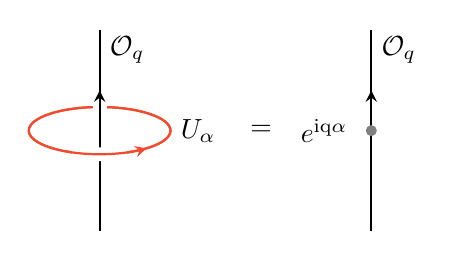
\begin{tikzpicture}[thick,scale=1.5]
  \pgfmathsetmacro{\wid}{.6}
  \pgfmathsetmacro{\toph}{.2}
  \pgfmathsetmacro{\ll}{1.7}
  \begin{knot}[
    %draft mode=crossings,
    clip width=2.5,
    flip crossing=2]
    %\strand[color=TopOp,arrow at={.4}{},draw,save path=\ug] (-{\wid},0) arc (-180:180:{\wid} and \toph);
    \strand[color=TopOp,draw,save path=\ug] (-{\wid},0) arc (-180:180:{\wid} and \toph);
    %\strand[arrow at={.55}{},draw] (0,-.5*\ll) -- ++(0,\ll);
    \strand[save path=\O] (0,-.5*\ll) -- ++(0,\ll);
  \end{knot}
  \draw[draw = none, arrow at={.4}{},color=TopOp] (-{\wid},0) arc (-180:180:{\wid} and \toph);
  \draw[draw = none, arrow at={.7}{}] (0,-.5*\ll) -- ++(0,\ll);
  \node[anchor=west] (Ua) at ({\wid},0) {$U_\alpha$};
  \node[anchor=west] at (0,\ll*.4) {$\mathcal{O}_q$};
  
  \begin{scope}[xshift=2.3cm]
    \draw[arrow at={.7}{}] (0,-.5*\ll) -- ++(0,\ll);
    \node[anchor=west] at (0,\ll*.4) {$\mathcal{O}_q$};
    \node (p) at (-.4,0) {$e^{\mathrm{iq \alpha}}$};
    \node[circle,inner sep=0,minimum size=4,fill=gray] at (0,0){};
  \end{scope}
  \node at ($(p)!.5!(Ua)$) {$=$};
\end{tikzpicture}
\end{document}
